% \yifan{Rerun evaluation with updated baselines. Update figures 5-8 and Tables 5 and 6.
% Table 7 should be good.}

% \yifan{Add results on Sparse Attn (with Deepseek 3.2); some multi-modal LLMs.}

\noindent\textbf{RQ1:}
Can \NAME{} accelerate end-to-end transformer-based model inference and outperform existing
tensor compilers and attention-specialized inference frameworks?
%Does \NAME{}'s performance benefit generalize to a variety of operators and input shapes?

\begin{figure*}[t!]
  \centering
  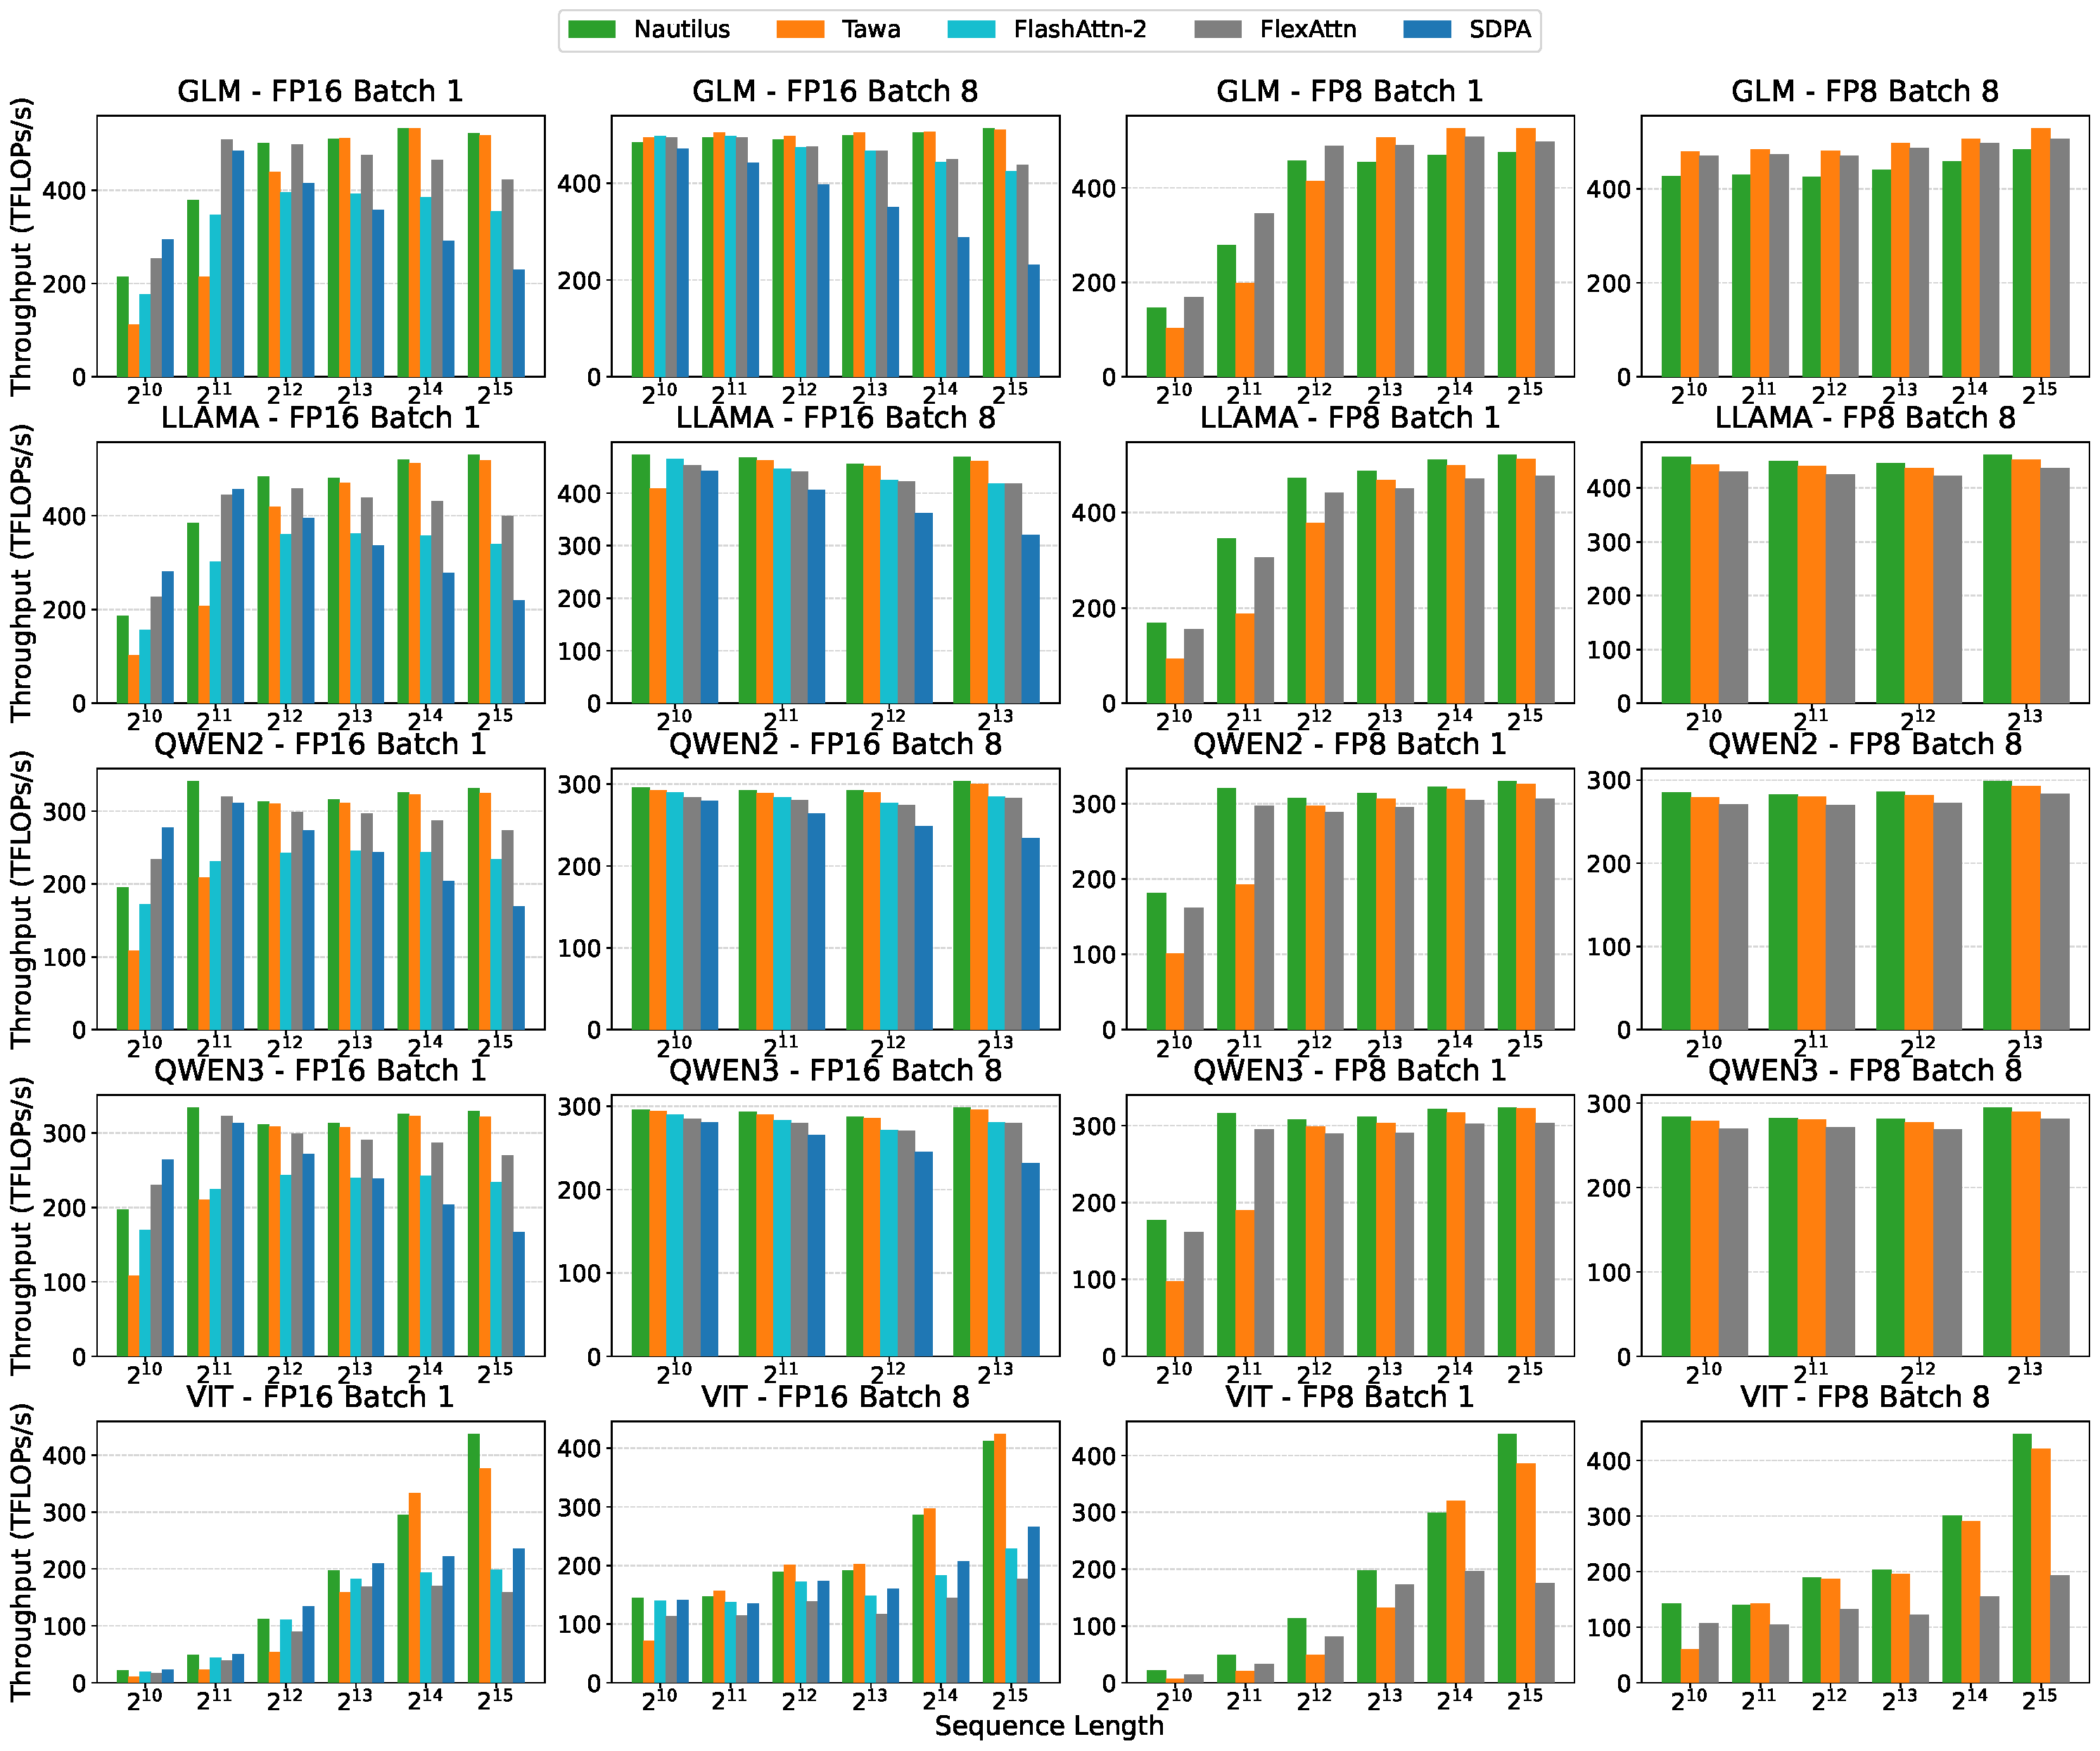
\includegraphics[width=0.9\textwidth]{figures/throughput_plot.pdf}
  \vspace{-1em}
  \caption{Throughput (TFLOPs/s) on GH200 across different models.
    We evaluate \NAME{} against baselines across five foundation models (GLM,
    Llama, Qwen2, Qwen3, ViT).
    The benchmarks cover FP16 and FP8 precisions with Batch Size 1 and 8, for sequence
  lengths ranging from 1k to 32k. }
  %\matei{This might be really annoying to do, but if it isn't too big a deal, I would
  % make it so that the bars are colored a bit differently (maybe with patterns) so they
  % can be easily distinguished in grayscale. I might also make the Nautilus color a bit
  % more distinct in some way to make it pop out more.}\yuchen{Of course we can change
  % the colors, any suggestions?}}
  \label{fig:gh200-throughput}
\end{figure*}

\begin{figure*}[t!]
  \centering
  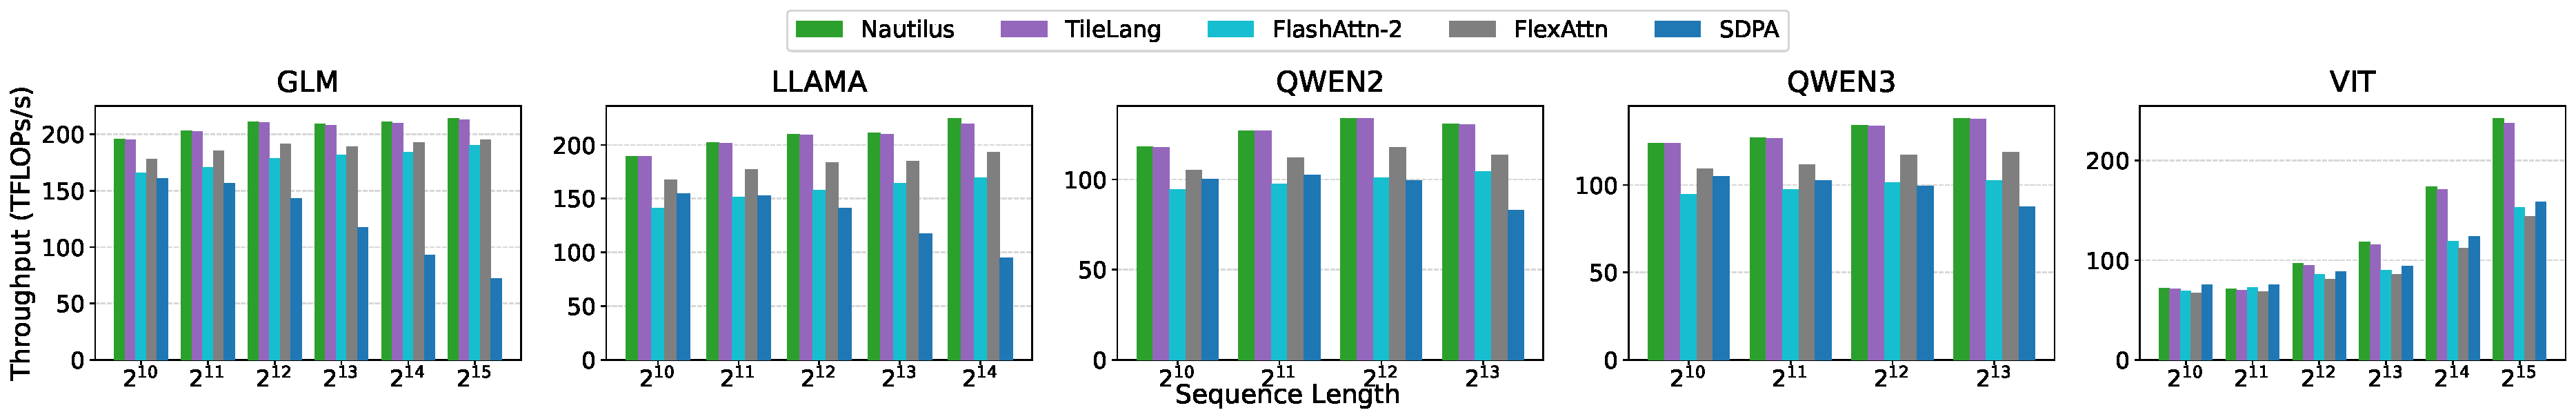
\includegraphics[width=0.95\textwidth]{figures/throughput_plot_5090.pdf}
  \vspace{-1em}
  \caption{Throughput (TFLOPs/s) on RTX 5090 across different models.
    We evaluate \NAME{} against baselines across five foundation models (GLM,
    Llama, Qwen2, Qwen3, ViT).
    The benchmarks cover sequence lengths ranging from 1k to 32k.
    % \sasa{How do we distinguish between batch 1 and 4?}
  }
  \label{fig:5090-throughput}
\end{figure*}

\noindent\textbf{RQ2:}
Can \NAME{} generate kernels that surpass the performance of kernels from existing tensor compilers?

\noindent\textbf{RQ3:}
Can \NAME{} generate kernels that have comparable performance to manually optimized
kernels in inference frameworks, which represent today's state of the art?

\noindent\textbf{RQ4:}
Ablation studies: How much do components of \NAME{} contribute to the performance of
\NAME{}'s attentions?

\subsection{End-to-End Model Inference}
\label{sec:eval-e2e}

\begin{table}[b!]
  \centering
  \small
  \setlength{\tabcolsep}{2.5pt}
  \caption{Geomean of relative throughput of \NAME{} against baselines on GH200
  across sequence lengths and batch sizes.}
  \label{tab:rq1-summary}
  \def\dgbox{\diagbox[width=6em, height=2.5em]{Model}{Method}}
  \renewcommand{\arraystretch}{0.93}
  \begin{tabular}{l|cccccc}
    \toprule
    \dgbox & Flash-2 & Flex & SDPA & Tawa & Flex-FP8 & Tawa-FP8 \\
    \midrule
    GLM     & 1.17 & 1.03 & 1.33 & 1.11 & 1.07 & 1.16 \\
    LLAMA   & 1.23 & 1.06 & 1.26 & 1.18 & 1.08 & 1.17 \\
    QWEN2   & 1.20 & 1.05 & 1.20 & 1.12 & 1.07 & 1.13 \\
    QWEN3   & 1.21 & 1.05 & 1.21 & 1.12 & 1.06 & 1.13 \\
    VIT     & 1.28 & 1.54 & 1.15 & 1.28 & 1.59 & 1.43 \\
    \bottomrule
    \textbf{Average} & 1.22 & 1.13 & 1.23 & 1.16 & 1.16 & 1.20 \\
    \bottomrule
  \end{tabular}\vspace{-.03in}
\end{table}

\textbf{Overall Trends.}
% \sasa{Aren't we talking about throughput here?}
To answer RQ1, we evaluate \NAME{} on two hardware generations: GH200 (Hopper) and RTX
5090 (Blackwell), using five representative foundation models:
GLM~\cite{du2022glmgenerallanguagemodel}, Llama2~\cite{touvron2023llama2openfoundation},
Qwen2~\cite{yang2024qwen2technicalreport}, Qwen3~\cite{yang2025qwen3technicalreport}, and
ViT~\cite{dosovitskiy2021imageworth16x16words}.
Table~\ref{tab:rq1-summary} and Table~\ref{tab:rq1-summary-5090} present the averaged
relative throughput of \NAME{} relative to state-of-the-art baselines including both
vendor-optimized libraries (FlashAttention-2, SDPA) and compiler-based approaches
(FlexAttn, Tawa~\cite{tawa}), where each cell represents the geometric mean over varying
sequence lengths and batch sizes.

Across the five representative foundation models in Table~\ref{tab:rq1-summary}, \NAME{}
achieves consistent performance gains in both FP16 and FP8 regimes.
In the FP16 setting, \NAME{} achieves an average speedup of $1.22\times$ over
FlashAttention-2 and $1.23\times$ over SDPA.
The performance advantage is most pronounced on the ViT architecture, where \NAME{}
achieves up to $1.54\times$ speedup against FlexAttn.
In the FP8 precision, \NAME{} shows improvements with an average speedup of $1.16\times$
over FlexAttn (FP8) and $1.20\times$ over Tawa (FP8).

On the RTX 5090 platform (Table~\ref{tab:rq1-summary-5090}), \NAME{} continues achieving
higher relative throughput.
In the FP16 setting, \NAME{} achieves an average relative throughput of $1.26\times$ over
FlashAttention-2 and $1.42\times$ over SDPA.
% Similar to the GH200 results, the gains are substantial on the ViT architecture, where
% \NAME{} outperforms FlexAttention by $1.85\times$ and SDPA by $1.83\times$.
Compared to the TileLang baseline, \NAME{} shows a slight improvement, since \NAME{}
automatically selects TileLang as the optimal backend on the RTX 5090 architecture, and
uses the auto-scheduler and auto-tuner to improve kernel performance \mbox{beyond the
default configurations.}

\begin{table}[t!]
  \centering
  \small
  \setlength{\tabcolsep}{6.5pt}
  \caption{Geometric mean of relative throughput of \NAME{} against baselines on RTX 5090
  across sequence lengths.}
  \label{tab:rq1-summary-5090}
  \def\dgbox{\diagbox[width=6em, height=2.5em]{Model}{Method}}
  \renewcommand{\arraystretch}{0.93}
\begin{tabular}{l|cccc}
  \toprule
  \dgbox & Flash-2 & Flex & SDPA & TileLang \\
  \midrule
  GLM     & 1.16 & 1.10 & 1.74 & 1.01 \\
  LLAMA   & 1.32 & 1.14 & 1.59 & 1.01 \\
  QWEN2   & 1.28 & 1.14 & 1.33 & 1.00 \\
  QWEN3   & 1.32 & 1.15 & 1.33 & 1.00 \\
  VIT     & 1.23 & 1.30 & 1.18 & 1.02 \\
  \midrule
  \textbf{Average} & 1.26 & 1.16 & 1.42 & 1.01 \\
  \bottomrule
\end{tabular}
\end{table}

Figure~\ref{fig:gh200-throughput} and Figure~\ref{fig:5090-throughput} report the
detailed throughput for these models across varying sequence lengths
($1k$ to $32k$) and batch sizes, where the y-axis shows the throughput in TFLOPs per second.
\NAME{} consistently outperforms baselines because its auto-scheduler and auto-tuner
identify optimized parameters for every specific workload, whereas baselines rely on
static rules/configs.

Similarly, \NAME{} achieves greater throughput gains on ViT than on LLMs.
This is because ViT involves less common attention configurations, with fewer
layers, fewer attention heads, and smaller hidden dimensions, which the
baselines often do not optimize well. \NAME{}, instead, generates efficient
kernel optimizations for these workloads.
%\matei{Grammatically, the end of this paragraph sounds a bit weird. Normally, I'd
% suggest something but I am too tired so I will recommend asking someone who has a bit
% more sleep.} \yuchen{Further modified}

\begin{figure*}[t!]
  \centering
  % First Row: GH200 FP16
  \begin{subfigure}[b]{0.95\textwidth}
    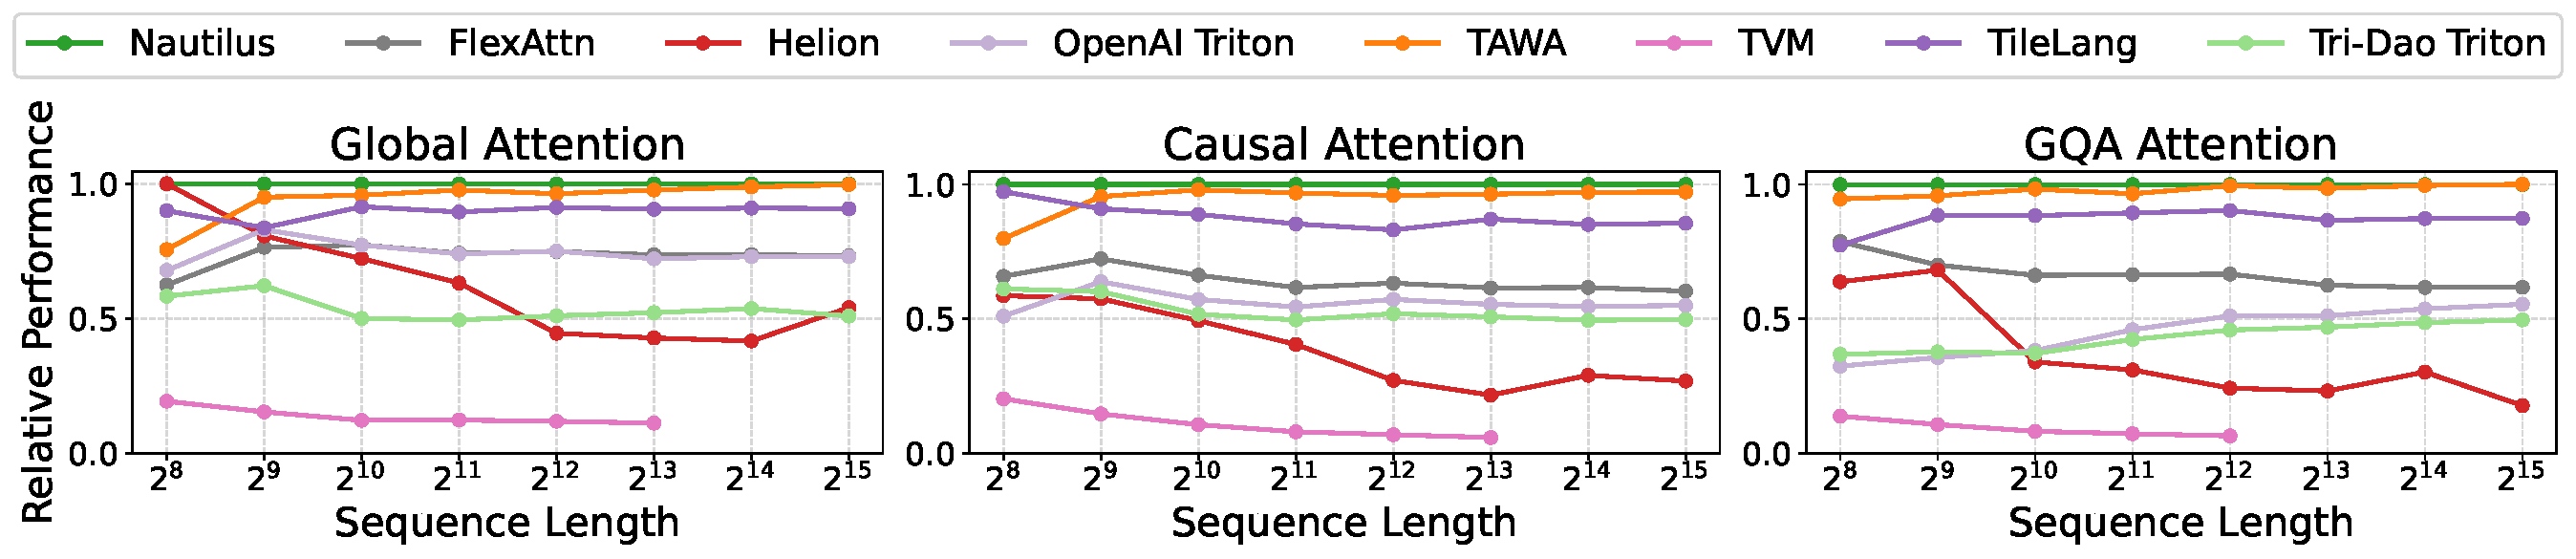
\includegraphics[width=\textwidth]{figures/gh200-fp16-tc1.pdf}
    \vspace{-1.7em}
    \caption{GH200: FP16 performance (higher is better).}
    \label{fig:gh200-fp16-tc}
  \end{subfigure}

  % Second Row: GH200 FP8
  \begin{subfigure}[b]{0.95\textwidth}
    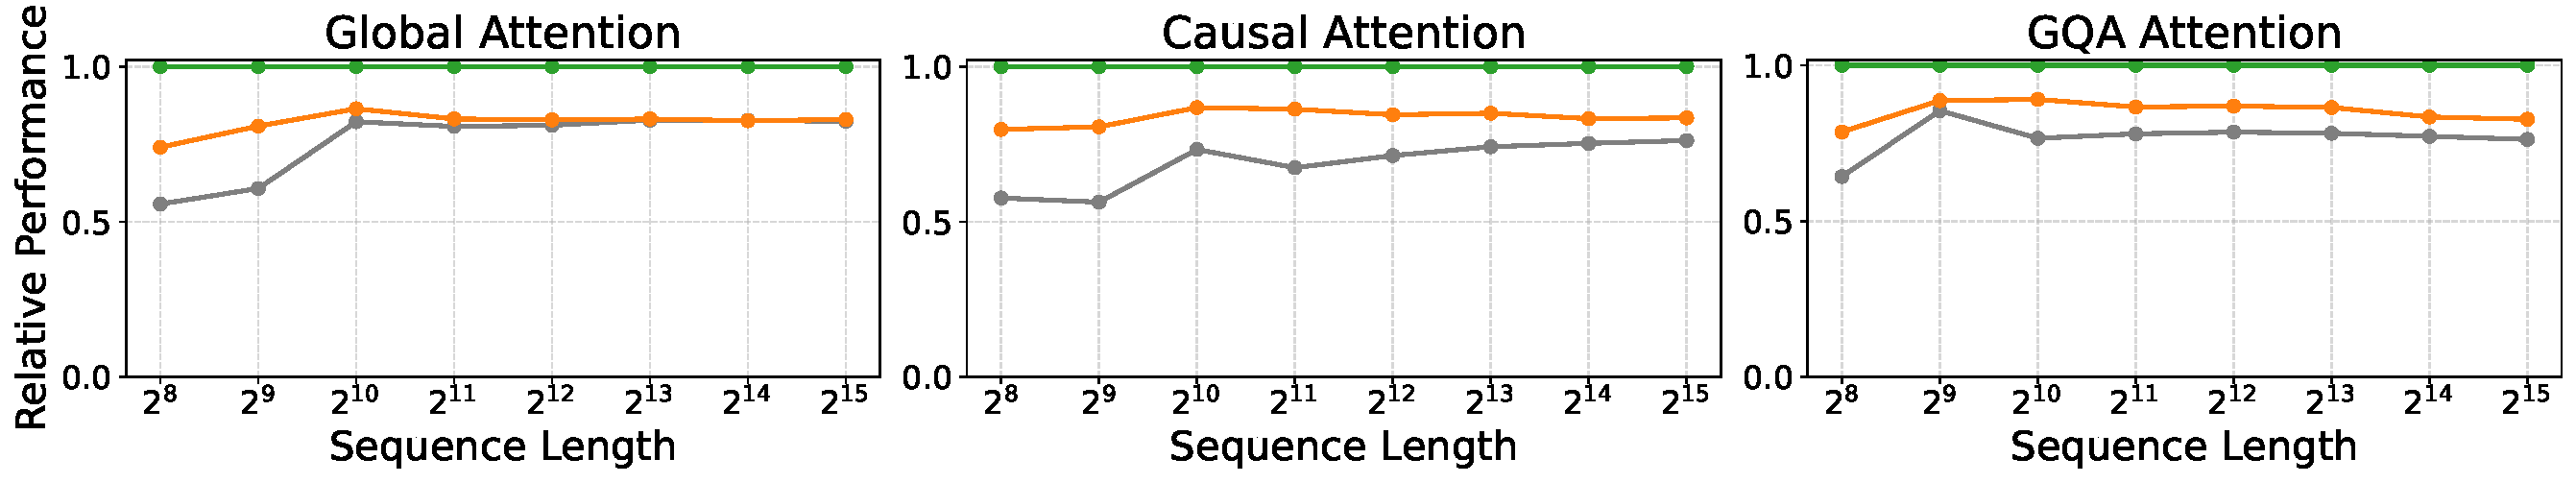
\includegraphics[width=\textwidth]{figures/gh200-fp8-tc1.pdf}
    \vspace{-1.7em}
    \caption{GH200: FP8 performance (higher is better).}
    \label{fig:gh200-fp8-tc}
  \end{subfigure}

  % Third Row: RTX 5090 FP16 (New)
  \begin{subfigure}[b]{0.95\textwidth}
    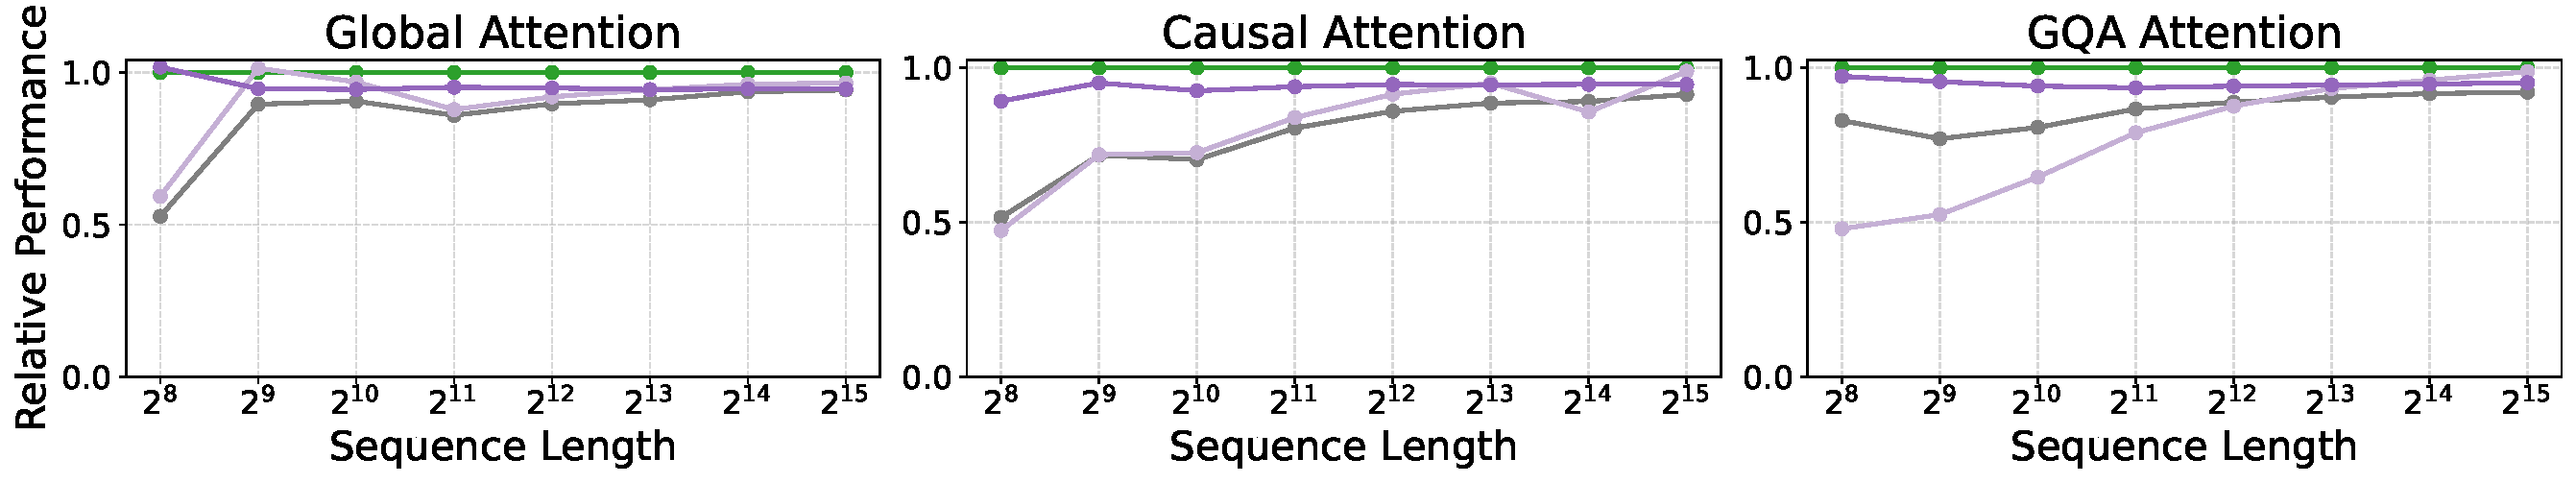
\includegraphics[width=\textwidth]{figures/rtx5090-fp16-tc1.pdf}
    \vspace{-1.7em}
    \caption{RTX 5090: FP16 performance (higher is better).}
    \label{fig:rtx5090-fp16-tc}
  \end{subfigure}

  \caption{Performance of \NAME{} kernels vs. kernels by other tensor compilers on GH200
    and RTX 5090 platforms.
  The y-axis shows relative performance of all compilers normalized to \NAME{} for each setup.}
  \vspace{-.1in}
  \label{fig:compiler-prefill-ablation}
\end{figure*}



\subsection{Detailed Kernel-level Latency Evaluation}

Figure~\ref{fig:compiler-prefill-ablation} illustrates the relative performance of
\NAME{} against leading tensor compilers across three attention-based operators on GH200
and RTX 5090 platforms.
Each subfigure reports the performance of baselines normalized to \NAME{} (y-axis) over
varying input sequence lengths (x-axis).
On the GH200 platform, \NAME{} achieves the best performance in the majority of setups.
At short sequence lengths, our auto-scheduler and auto-tuner gain a significant advantage
over Tawa by automatically selecting the faster TileLang~\cite{tilelang} backend and
tuning parameters towards smaller block sizes and fewer pipeline stages.
%
For instance, on short sequences, \NAME{} selects a lighter $64 \times 128$ tile size
with 4 warps, while Tawa defaults to a heavy $128 \times 128$ size with 8 warps.
This adaptability provides even larger benefits for FP8 precision. \NAME{} adjusts
parameters such as pipeline stages from 1 to 4 based on sequence length which the
performance of models in FP8 relies heavily on, so \NAME{} can achieve bigger performance
improvements compared to FP16.
%
On the RTX 5090, \NAME{} consistently outperforms baselines, with larger speedups
observed on longer sequences where our autoscheduler selects the rolling update
optimization to overcome TileLang.
In FP8 precision setups (Figure \ref{fig:gh200-fp8-tc}), \NAME{} demonstrates a
significant advantage, achieving \mbox{approximately} 20\% improvement on average over the
strongest baselines, enabled by the optimized \mbox{configurations} identified by our auto-tuner.
%
Our auto-tuner shows hardware adaptability by adjusting the search space parameters, e.g., block sizes, to accommodate the limited shared \mbox{memory of the RTX 5090.}

We do not show Neptune results since Neptune's performance is limited by Triton's performance,
due to being tied to Triton for code generation, which struggles to generate efficient code for these
operators on Hopper and Blackwell.
Our measurements show Neptune's speed is 0.5x-0.8x of that of Tawa or TileLang. %Table~\ref{tab:neptune_perf}
% show that Neptune is slower than other baselines.
This result indicates that the main bottleneck is backend code generation rather than schedule quality. Our results suggest that the schedules found by \NAME{} are already competitive with the manually written schedules used by the Neptune developers, and that the remaining gap comes from Triton's lower code quality on these platforms.
% \sasa{Separate: Somewhere need to say that our schedules are as good as those the Neptune developers manually wrote. }

% \sasa{What can we say here about specific cases? }

% \sasa{How can we relate the speedup to the success of our transformations/scheduling? }

% \sasa{We should also say why Neptune is not applicable here!! (Slow triton!)}

%\sasa{We should include some details about the schedules, which Matei mentioned in the
% slack "GQA and prefill attention are different in that GQA has an extra loop and some
% reshaping (which is merged into a block present in prefill-generated schedules). Other
% than that, only compiler flags/annotations differ at my level." Ofc emphasize the diffs
% and variety across schedules...}
% \sasa{Mention if there is even a small difference between schedules for GPU generations.}

\subsection{\NAME{} vs Manually-Written Kernels}

% Figure~\ref{fig:libs-prefill-comparison} compares \NAME{} against heavily optimized,
% hand-written kernel libraries on GH200 and RTX 5090 platforms.
% Across both hardware generations, \NAME{} generates kernels that consistently match or
% exceed the performance of state-of-the-art vendor libraries.
% %On GH200,
% \NAME{} matches the performance of the highly optimized cuDNN kernel.
% While hand-written libraries like cuDNN can be slightly faster in specific cases, they
% require intensive manual tuning that is difficult to maintain across different operators
% and hardware generations.

Appendix~\ref{sec:vendor-libs} compares \NAME{} against heavily optimized,
hand-written vendor libraries on GH200 and RTX 5090.
Across both hardware generations, \NAME{} matches or exceeds the performance of
state-of-the-art vendor libraries in most setups, and remains close to the highly
optimized cuDNN kernels in the remaining cases.

% For instance, supporting a new feature like SoftCap or ALiBi bias in cuDNN often
% requires waiting for vendor updates or accepting performance loss from unfused operations.
% In contrast, \NAME{} can automatically generate optimized, fused kernels for such custom variants.
%On the RTX 5090 (Blackwell) architecture, \NAME{} maintains consistent high performance
% across the entire range of configurations, matching or outperforming the
% \mbox{strongest hand-tuned baselines.}

% \sasa{We need a clear case here and explanation that even when cudnn is sometimes
% faster, it is pain to maintain and hand-tune...}

\subsection{Numerical Stability}
In Appendix~\ref{sec:num-stab}, we evaluate the numerical behavior of \NAME{}-generated kernels.
Using realistic Qwen2.5 inputs and an FP64 attention implementation as reference, \NAME{} shows numerical error comparable to Tri-Dao Attention and FlexAttention across PF Global, PF Causal, and PF GQA.
Averaged across the three operators, \NAME{} achieves an RMS absolute error of $4.96\times 10^{-5}$, compared with $4.90\times 10^{-5}$ for Tri-Dao and $5.02\times 10^{-5}$ for FlexAttention.
% \sasa{SAY WHICH Appendix. Also mention the averages in text. }



\subsection{Ablation Studies}

\begin{table}[t]
  \centering
  \caption{Ablation study of \NAME{}'s latency}
  \label{tab:ablation}
  \begin{tabular}{lc}
    \toprule
    \textbf{Configuration} & \textbf{Latency ($\mu s$)} \\
    \midrule
    \NAME{} (Full System) & 7.43 \\
    w/o Auto-tuning & 9.09 \\
    w/o Auto-tuning \& Expression Rewriting & 9.45 \\
    w/o Auto-scheduling & 10.93 \\
    \bottomrule
  \end{tabular}
\end{table}

To understand the importance of each component of \NAME{},
we perform ablation studies on the performance of \NAME{}'s kernels.
We select the Global attention operator with sequence length 256 on GH200.
Table \ref{tab:ablation} shows the results of this experiment.
The full \NAME{} system achieves the latency of 7.43 $\mu s$.
Disabling components progressively increases latency: removing the auto-tuner causes a
significant drop to 9.09$\mu$s. This shows the importance of parameter tuning.
Additionally disabling expression rewriting leads to further degradation to 9.45 $\mu s$.
Finally, the configuration with no auto-scheduling yields the highest latency of 10.93 $\mu s$.

\noindent\textbf{Autoscheduler Statistics.} \NAME{}'s auto-scheduling search is
relatively fast and finishes within a minute in most cases due to aggressive pruning. 
The auto-tuner takes a bit longer, taking from seconds to 10
minutes, as it needs to compile and runs many kernels.
\NAME-generated schedules contain a variety of different optimizations. GQA has several
reshape and broadcast operations added with respect to the base prefill attention, in
addition to an \mbox{extra loop nest.}
